 

\index{Image Correspondences}

\section{Image Correspondences}

\subsection{Corners}

There are several techniques to track an object. If there is information about the object of interest the problem 
can be simplified using this information to restrict the search space, for example to certain color or shape.
 By the other hand if the object to track is unknown, it is necessary to find a more general feature, that is 
more likely to be found on the unknown interest objects. The corners are good features for this purpose. A corner 
is a point on the image where there are gradient variations on two orthogonal directions.

The most common definition of a corner is gived by Harris corners method.

Consider a function E(u,v), to measure a difference between the pixels of a window (a region of the image) and 
a window shifted (u,v) units:

\begin{equation}
E(u,v) = \sum\limits_{x,y} { w(x,y) [I(x + u, y +v) - I(x,y)]^2  }\ .
\label{eq:harris1}
\end{equation}

We loop over a neighborhood defined by different values of (x,y) and calculate 
the difference of each pixel located at (x,y) with some other pixel located at (x+u,y+v). 
The function w(x,y) defines the window where we are working, in the case of a square windows, 
it has values 1 for pixels inside the window and 0 for other pixels. In the case of a circular 
window a Gaussian function can be used. 

E(u,v) will have bigger values when the window is centered in a corner. For this reason we want 
to detect when E(u,v) is maximum. With this purpose on mind, we can express $I(x + u, y +v)$ in a more convenient
 way using a Taylor expansion:

$$
I(x+u,y +v) = I(x,y) + I_xu + I_yv + Higher Order Terms \ ,
$$ 

\noindent where 

$$
I_x = \frac{\partial{I(x,y)}}{\partial{x}}\ ,
$$

$$
I_y = \frac{\partial{I(x,y)}}{\partial{y}}\ .
$$

Then we can use the following approximation:

$$
I(x+u,y +v) \approx I(x,y) + I_xu + I_yv\ ,
$$

$$
I(x+u,y +v) \approx I(x,y) + \begin{bmatrix} I_x & I_y \end{bmatrix} \begin{bmatrix} u \\ v \end{bmatrix}\ ,
$$ 

\noindent replacing this in \ref{eq:harris1} we get:

$$
E(u,v) \approx \sum\limits_{x,y} { w(x,y) [I(x,y)  + \begin{bmatrix} I_x & I_y \end{bmatrix} \begin{bmatrix} u \\ v \end{bmatrix} - I(x,y)]^2  }\ ,
$$

$$
E(u,v) \approx \sum\limits_{x,y} { w(x,y) [\begin{bmatrix} I_x & I_y \end{bmatrix} \begin{bmatrix} u \\ v \end{bmatrix} ]^2  }\ ,
$$

$$
E(u,v) \approx \begin{bmatrix} u & v \end{bmatrix} \sum\limits_{x,y} w(x,y) \underbrace{\begin{bmatrix} {I_x}^2 & I_x I_y \\ I_x I_y & {I_y}^2 \end{bmatrix}}_{H} \begin{bmatrix} u \\ v \end{bmatrix}\ .
$$


Eigenvalues of H can be used to detect corners. When both eigenvalues have large magnitude, the window contains a corner. If just one 
eigenvalue has large magnitude we have an edge and if both eigenvalues have small magnitude we have a plain surface.

Once we have corners, we can find the movement of each corner between two successive images using Optical Flow. The objective 
is to find correspondences (common points) between the two images.

\subsection{Optical Flow}

The optical flow methods are used to calculate motion between two successive image captures which are taken
 at two different times: $t$ and $t + \Delta t$.

These methods have two main assumptions about the frames \cite{sonka2007}:

\begin{enumerate}
\item The observed brightness of any object point is constant over time.
\item Nearby points in the image plane move in a similar manner (velocity smoothness).
\end{enumerate}

\begin{figure}[h!]
\begin{center}
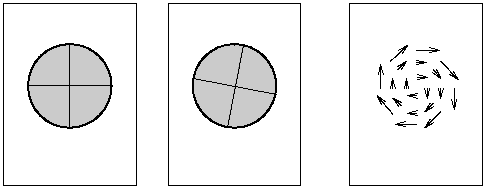
\includegraphics[scale=0.6]{images/oflow}
\caption{Image at time $t$, image at time $t + \Delta t$ and optical flow.}
\label{fig:oflow}
\end{center}
\end{figure}

There are two kinds of optical flow: dense and sparse. Dense optical flow means to calculate a direction vector for each pixel of the image and sparse optical flow is calculate direction vector just for those pixels of the image 
who satisfy certain conditions.

Dense optical flow is computationally expensive and it is difficult to find the direction vector 
for plain color areas. For example in an image of a white paper or a wall
there are a lot of pixels with the same properties and it is necessary to perform some kind of interpolation to give a direction vector
 to each one of these pixels. 
By the other hand, sparse optical flow just consider pixels with more odds of matching between the two frames.

\subsection{Lukas-Kanade Method}
\label{sec:oflow}

The Lukas-Kanade method is a sparse optical flow method, that 
uses a search window for each pixel of interest and assume that all the pixels 
inside the search window have the same direction vector.


We have two images: $I(x,y,t)$ and $I(x,y,t+\Delta t)$.
If optical flow conditions are meet :

\begin{equation}
\label{eq:oflowrel}
I(x + \Delta x,y + \Delta y, t + \Delta t) = I(x,y,t)\ .
\end{equation}

We can express $I(x + \Delta x, y + \Delta y, t + \Delta t)$ using Taylor series as:

\begin{equation}
\label{eq:oflowtaylor}
I(x + \Delta x, y + \Delta y, t + \Delta t) = I(x,y,t) + \frac{\partial I}{\partial y} \Delta y + \
 \frac{\partial I}{\partial x} \Delta x  + \frac{\partial I}{\partial t} \Delta t + Higher Order Terms \ .
\end{equation}

If we combine \ref{eq:oflowrel} and \ref{eq:oflowtaylor} we obtain the general optical flow equation :


$$ I(x,y,t) + \frac{\partial I}{\partial y} \Delta y + \
 \frac{\partial I}{\partial x} \Delta x  + \frac{\partial I}{\partial t} \Delta t + Higher Order Terms = I(x,y,t)\ , $$


$$ \frac{\partial I}{\partial y} \Delta y + \
 \frac{\partial I}{\partial x} \Delta x  + \frac{\partial I}{\partial t} \Delta t \approx 0 \hspace{0.5cm} \backslash \cdot \frac{1}{\Delta t}\ ,  $$


$$ \frac{\partial I}{\partial y} \frac{\Delta y}{\Delta t} + \
 \frac{\partial I}{\partial x} \frac{\Delta x}{\Delta t}  + \frac{\partial I}{\partial t}  \approx 0 \ , $$


\noindent let :

$$ V_x = \frac{\Delta x}{\Delta t}\ , $$
$$ V_y = \frac{\Delta y}{\Delta t}\ , $$
$$ I_x = \frac{\partial I}{\partial x}\ ,$$
$$ I_y = \frac{\partial I}{\partial y}\ ,$$

\noindent and finally we get :

$$ I_x V_x + I_y V_y = -I_t \ ,$$

\begin{equation}
\label{eq:oflowgeneral}
\nabla{\vec{I}} \cdot \vec{V} = -I_t \ .
\end{equation}

We have an equation with two unknowns $V_x$ and $V_y$, we can't solve it without additional restrictions.

The Lukas-Kanade method assumes that all the pixels inside a window satisfy this equation for the same 
values of $V_x$ and $V_y$. Thus, if we have a $5\times5$ window, we have 25 equations with two unknowns :

$$
\begin{bmatrix}
I_x(p1) & I_y(p1) \\
I_x(p2) & I_y(p2) \\
... & ... \\
I_x(p25) & I_y(p25)\\
\end{bmatrix}  \ ,
\begin{bmatrix}
V_x \\
V_y\\
\end{bmatrix}
=
-\begin{bmatrix}
I_t(p1) \\
I_t(p2) \\
...     \\
I_t(p25) 
\end{bmatrix} \ ,
$$

where $p_1, p_2, ..., p_{25}$ are pixel 1, pixel 2, etc.

Let 

$$
A = 
\begin{bmatrix}
I_x(p1) & I_y(p1) \\
I_x(p2) & I_y(p2) \\
... & ... \\
I_x(p25) & I_y(p25)\\
\end{bmatrix}  \ ,
$$

$$
x=
\begin{bmatrix}
V_x \\
V_y\\
\end{bmatrix} \ ,
$$

$$
b=
-\begin{bmatrix}
I_t(p1) \\
I_t(p2) \\
...     \\
I_t(p25) 
\end{bmatrix} \ .
$$

\noindent Then we have the classical problem :

$$ 
Ax = b\ .
$$

\noindent A solution can be obtained by the least squares, using partial derivatives of the unknowns and equating to zero, the following expression
 is obtained:

$$
x = (A^T A)^{-1} A^T b \ .
$$


\noindent $A^T A$ will be invertible depending on the pixels of the image. Even if $A^T A $ is invertible, 
if its values are very small it can be ill conditioned. For this reason it is necessary to check the eigenvalues of $A^T A$, if they are zero or very small, then it is not possible to find a solution.

In order to increment the odds of obtaining a solution the Lukas Kanade method works only in the corners detected on the image, because corners are better points to be tracked.

\subsection{Speeded Up Robust Features}
\label{sec:surf}

The Speeded Up Robust Features (SURF) algorithm finds image features looking for strong responses in two orthogonal directions, in order to detect points that are strong to rotation and translation transformations. For this purpose the determinant of the Hessian matrix calculated for each pixel is used:


$$
H = \begin{bmatrix} I_{xx} & I_x I_y \\ I_x I_y & I_{yy} \end{bmatrix} \begin{bmatrix} u \\ v \end{bmatrix} \ ,
$$

$$
det(H) = I_{xx} I_{yy} - I_{xy}^2\ .
$$


\noindent The second order partial derivatives are approximated using just a box filter, in other words 
summing and subtracting pixel values instead of using the classical Gaussian weighing. 

\begin{figure}[!h]
\begin{center}
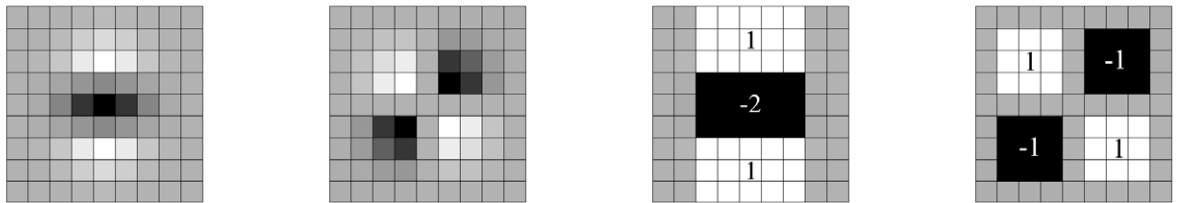
\includegraphics[scale=0.35]{images/surf_mask}
\caption{Left to right: the discretized and cropped Gaussian second order partial derivatives 
in y-direction and xy-direction, and approximations using box filters. 
Grey regions are equal to zero. Image extracted from \cite{Bay06surf}.}
\end{center}
\end{figure}

This filter is applied to each pixel of the image, obtaining the value $det(H)$ for each one of the pixels. 

When it is necessary to extract features from an image, the image  usually is scaled to different sizes (scale-space) in order 
to find image structures 
at different scales. SURF algorithm instead of scale the image, scales the filter applied to the 
image, increasing the speed of the calculations in one order of magnitude.

\begin{figure}[!h]
\begin{center}
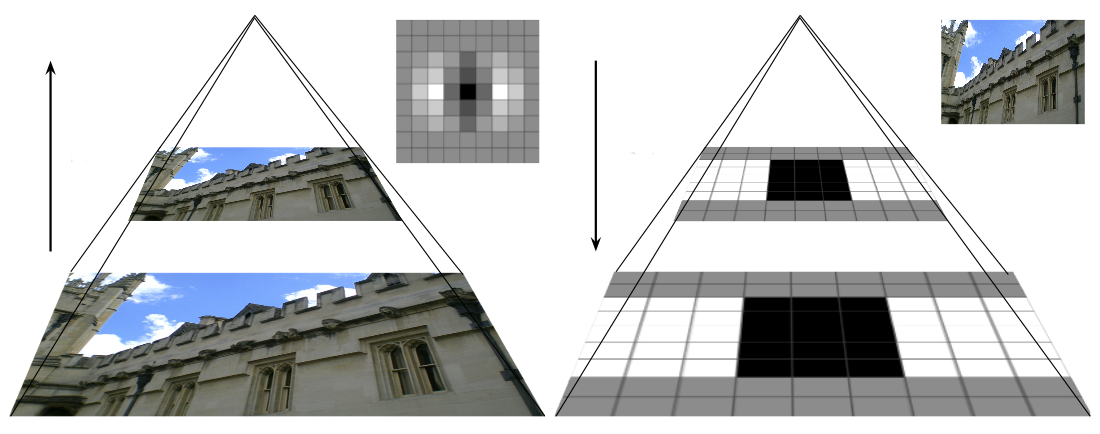
\includegraphics[scale=0.35]{images/surf_scale}
\caption{Left to right: traditional approach to produce scale-space, scaling image and applying Gaussian filter. SURF approach to produce scale-space, scaling the filter and maintaining the image size. Image extracted from \cite{miguel}.}
\end{center}
\end{figure}


In order to find interest points a non-maximal suppression is applied, in order to maintain only points above certain threshold. 

\begin{figure}[H]
\begin{center}
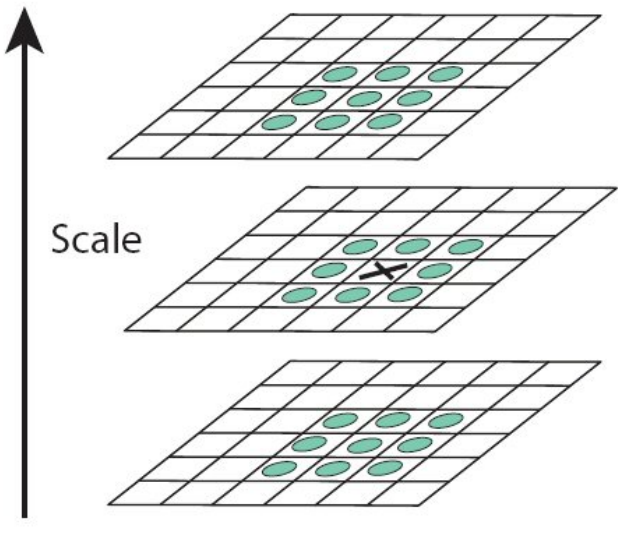
\includegraphics[scale=0.28]{images/surf_nb}
\caption{Non-Maximal Suppression. The pixel marked X is selected as a maximum if it is greater than the 
surrounding pixels on its interval and intervals above and below. Image extracted from \cite{OpenSURF}.}
\end{center}
\end{figure}

At the end of this step a set of interest points is obtained. Then an interpolation is applied, in order to find the location 
at sub-pixel accuracy.

Once the set of points is calculated, a descriptor to each point is generated. The descriptor is calculated relative to a dominant 
orientation, in order to reach rotation invariance.
 
The following features are used to describe a point $v=\{dx,dy,|dx|.|dy|\}$ this features are calculated in several regions 
around the interest point. Obtaining a vector of 64 components that is normalized to reduce the effect of changes in the image 
intensities. A complete explanation of how this algorithm works can be found in \cite{OpenSURF}


